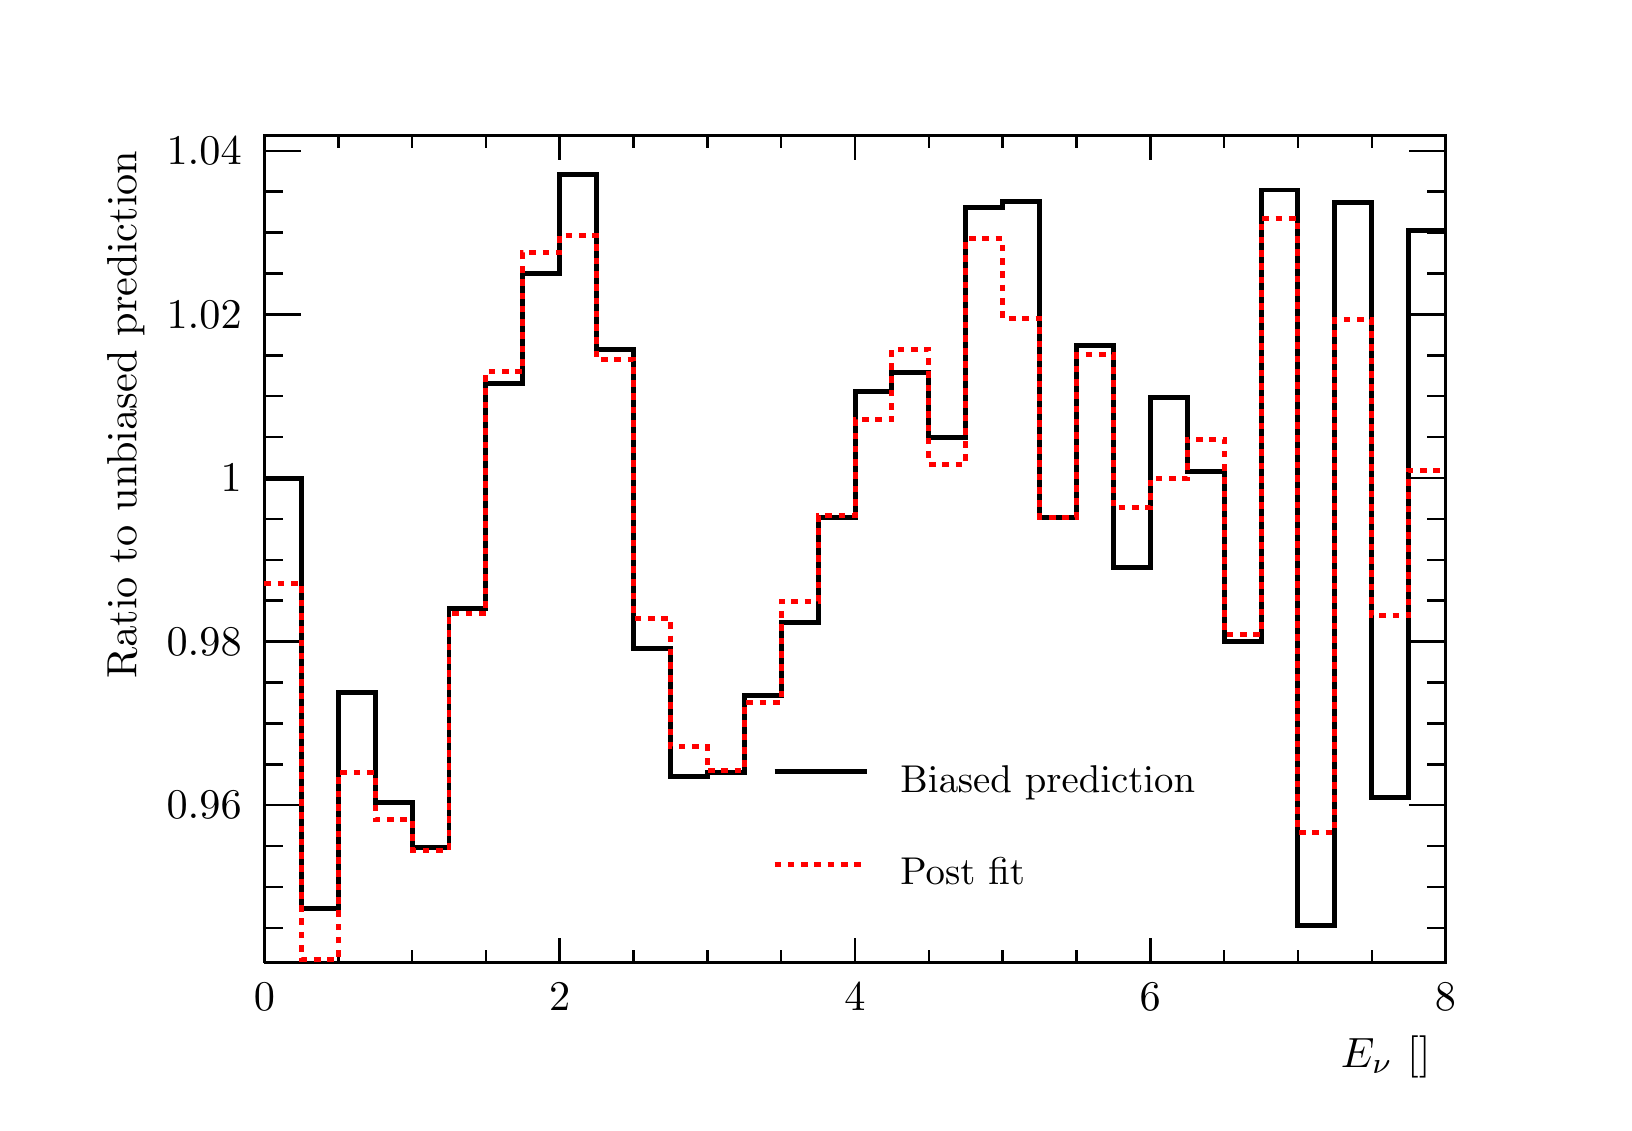
\begin{tikzpicture}
\pgfdeclareplotmark{cross} {
\pgfpathmoveto{\pgfpoint{-0.3\pgfplotmarksize}{\pgfplotmarksize}}
\pgfpathlineto{\pgfpoint{+0.3\pgfplotmarksize}{\pgfplotmarksize}}
\pgfpathlineto{\pgfpoint{+0.3\pgfplotmarksize}{0.3\pgfplotmarksize}}
\pgfpathlineto{\pgfpoint{+1\pgfplotmarksize}{0.3\pgfplotmarksize}}
\pgfpathlineto{\pgfpoint{+1\pgfplotmarksize}{-0.3\pgfplotmarksize}}
\pgfpathlineto{\pgfpoint{+0.3\pgfplotmarksize}{-0.3\pgfplotmarksize}}
\pgfpathlineto{\pgfpoint{+0.3\pgfplotmarksize}{-1.\pgfplotmarksize}}
\pgfpathlineto{\pgfpoint{-0.3\pgfplotmarksize}{-1.\pgfplotmarksize}}
\pgfpathlineto{\pgfpoint{-0.3\pgfplotmarksize}{-0.3\pgfplotmarksize}}
\pgfpathlineto{\pgfpoint{-1.\pgfplotmarksize}{-0.3\pgfplotmarksize}}
\pgfpathlineto{\pgfpoint{-1.\pgfplotmarksize}{0.3\pgfplotmarksize}}
\pgfpathlineto{\pgfpoint{-0.3\pgfplotmarksize}{0.3\pgfplotmarksize}}
\pgfpathclose
\pgfusepathqstroke
}
\pgfdeclareplotmark{cross*} {
\pgfpathmoveto{\pgfpoint{-0.3\pgfplotmarksize}{\pgfplotmarksize}}
\pgfpathlineto{\pgfpoint{+0.3\pgfplotmarksize}{\pgfplotmarksize}}
\pgfpathlineto{\pgfpoint{+0.3\pgfplotmarksize}{0.3\pgfplotmarksize}}
\pgfpathlineto{\pgfpoint{+1\pgfplotmarksize}{0.3\pgfplotmarksize}}
\pgfpathlineto{\pgfpoint{+1\pgfplotmarksize}{-0.3\pgfplotmarksize}}
\pgfpathlineto{\pgfpoint{+0.3\pgfplotmarksize}{-0.3\pgfplotmarksize}}
\pgfpathlineto{\pgfpoint{+0.3\pgfplotmarksize}{-1.\pgfplotmarksize}}
\pgfpathlineto{\pgfpoint{-0.3\pgfplotmarksize}{-1.\pgfplotmarksize}}
\pgfpathlineto{\pgfpoint{-0.3\pgfplotmarksize}{-0.3\pgfplotmarksize}}
\pgfpathlineto{\pgfpoint{-1.\pgfplotmarksize}{-0.3\pgfplotmarksize}}
\pgfpathlineto{\pgfpoint{-1.\pgfplotmarksize}{0.3\pgfplotmarksize}}
\pgfpathlineto{\pgfpoint{-0.3\pgfplotmarksize}{0.3\pgfplotmarksize}}
\pgfpathclose
\pgfusepathqfillstroke
}
\pgfdeclareplotmark{newstar} {
\pgfpathmoveto{\pgfqpoint{0pt}{\pgfplotmarksize}}
\pgfpathlineto{\pgfqpointpolar{44}{0.5\pgfplotmarksize}}
\pgfpathlineto{\pgfqpointpolar{18}{\pgfplotmarksize}}
\pgfpathlineto{\pgfqpointpolar{-20}{0.5\pgfplotmarksize}}
\pgfpathlineto{\pgfqpointpolar{-54}{\pgfplotmarksize}}
\pgfpathlineto{\pgfqpointpolar{-90}{0.5\pgfplotmarksize}}
\pgfpathlineto{\pgfqpointpolar{234}{\pgfplotmarksize}}
\pgfpathlineto{\pgfqpointpolar{198}{0.5\pgfplotmarksize}}
\pgfpathlineto{\pgfqpointpolar{162}{\pgfplotmarksize}}
\pgfpathlineto{\pgfqpointpolar{134}{0.5\pgfplotmarksize}}
\pgfpathclose
\pgfusepathqstroke
}
\pgfdeclareplotmark{newstar*} {
\pgfpathmoveto{\pgfqpoint{0pt}{\pgfplotmarksize}}
\pgfpathlineto{\pgfqpointpolar{44}{0.5\pgfplotmarksize}}
\pgfpathlineto{\pgfqpointpolar{18}{\pgfplotmarksize}}
\pgfpathlineto{\pgfqpointpolar{-20}{0.5\pgfplotmarksize}}
\pgfpathlineto{\pgfqpointpolar{-54}{\pgfplotmarksize}}
\pgfpathlineto{\pgfqpointpolar{-90}{0.5\pgfplotmarksize}}
\pgfpathlineto{\pgfqpointpolar{234}{\pgfplotmarksize}}
\pgfpathlineto{\pgfqpointpolar{198}{0.5\pgfplotmarksize}}
\pgfpathlineto{\pgfqpointpolar{162}{\pgfplotmarksize}}
\pgfpathlineto{\pgfqpointpolar{134}{0.5\pgfplotmarksize}}
\pgfpathclose
\pgfusepathqfillstroke
}
\definecolor{c}{rgb}{1,1,1};
\draw [color=c, fill=c] (0,0) rectangle (20,13.639);
\draw [color=c, fill=c] (3,1.77307) rectangle (18,12.2751);
\definecolor{c}{rgb}{0,0,0};
\draw [c,line width=0.9] (3,1.77307) -- (3,12.2751) -- (18,12.2751) -- (18,1.77307) -- (3,1.77307);
\definecolor{c}{rgb}{1,1,1};
\draw [color=c, fill=c] (3,1.77307) rectangle (18,12.2751);
\definecolor{c}{rgb}{0,0,0};
\draw [c,line width=0.9] (3,1.77307) -- (3,12.2751) -- (18,12.2751) -- (18,1.77307) -- (3,1.77307);
\draw [c,line width=1.8] (3,7.92661) -- (3.46875,7.92661) -- (3.46875,2.46016) -- (3.9375,2.46016) -- (3.9375,5.20191) -- (4.40625,5.20191) -- (4.40625,3.80739) -- (4.875,3.80739) -- (4.875,3.22978) -- (5.34375,3.22978) -- (5.34375,6.26977) --
 (5.8125,6.26977) -- (5.8125,9.1268) -- (6.28125,9.1268) -- (6.28125,10.5299) -- (6.75,10.5299) -- (6.75,11.775) -- (7.21875,11.775) -- (7.21875,9.56118) -- (7.6875,9.56118) -- (7.6875,5.76429) -- (8.15625,5.76429) -- (8.15625,4.13491) --
 (8.625,4.13491) -- (8.625,4.1814) -- (9.09375,4.1814) -- (9.09375,5.16368) -- (9.5625,5.16368) -- (9.5625,6.09716) -- (10.0312,6.09716) -- (10.0312,7.42544) -- (10.5,7.42544) -- (10.5,9.02799) -- (10.9688,9.02799) -- (10.9688,9.26414) --
 (11.4375,9.26414) -- (11.4375,8.43817) -- (11.9062,8.43817) -- (11.9062,11.3568) -- (12.375,11.3568) -- (12.375,11.4419) -- (12.8438,11.4419) -- (12.8438,7.42727) -- (13.3125,7.42727) -- (13.3125,9.61133) -- (13.7812,9.61133) -- (13.7812,6.78862) --
 (14.25,6.78862) -- (14.25,8.95342) -- (14.7188,8.95342) -- (14.7188,8.00443) -- (15.1875,8.00443) -- (15.1875,5.85361) -- (15.6562,5.85361) -- (15.6562,11.5844) -- (16.125,11.5844) -- (16.125,2.24935) -- (16.5938,2.24935) -- (16.5938,11.4198) --
 (17.0625,11.4198) -- (17.0625,3.87361) -- (17.5312,3.87361) -- (17.5312,11.0745) -- (18,11.0745);
\draw [c,line width=0.9] (3,1.77307) -- (18,1.77307);
\draw [c,line width=0.9] (3,2.07994) -- (3,1.77307);
\draw [c,line width=0.9] (3.9375,1.9265) -- (3.9375,1.77307);
\draw [c,line width=0.9] (4.875,1.9265) -- (4.875,1.77307);
\draw [c,line width=0.9] (5.8125,1.9265) -- (5.8125,1.77307);
\draw [c,line width=0.9] (6.75,2.07994) -- (6.75,1.77307);
\draw [c,line width=0.9] (7.6875,1.9265) -- (7.6875,1.77307);
\draw [c,line width=0.9] (8.625,1.9265) -- (8.625,1.77307);
\draw [c,line width=0.9] (9.5625,1.9265) -- (9.5625,1.77307);
\draw [c,line width=0.9] (10.5,2.07994) -- (10.5,1.77307);
\draw [c,line width=0.9] (11.4375,1.9265) -- (11.4375,1.77307);
\draw [c,line width=0.9] (12.375,1.9265) -- (12.375,1.77307);
\draw [c,line width=0.9] (13.3125,1.9265) -- (13.3125,1.77307);
\draw [c,line width=0.9] (14.25,2.07994) -- (14.25,1.77307);
\draw [c,line width=0.9] (15.1875,1.9265) -- (15.1875,1.77307);
\draw [c,line width=0.9] (16.125,1.9265) -- (16.125,1.77307);
\draw [c,line width=0.9] (17.0625,1.9265) -- (17.0625,1.77307);
\draw [c,line width=0.9] (18,2.07994) -- (18,1.77307);
\draw [anchor=base] (3,1.15931) node[scale=1.52731, color=c, rotate=0]{0};
\draw [anchor=base] (6.75,1.15931) node[scale=1.52731, color=c, rotate=0]{2};
\draw [anchor=base] (10.5,1.15931) node[scale=1.52731, color=c, rotate=0]{4};
\draw [anchor=base] (14.25,1.15931) node[scale=1.52731, color=c, rotate=0]{6};
\draw [anchor=base] (18,1.15931) node[scale=1.52731, color=c, rotate=0]{8};
\draw [anchor= east] (18,0.572837) node[scale=1.52731, color=c, rotate=0]{$E_{\nu}$ [\si{\GeV}]};
\draw [c,line width=0.9] (3,12.2751) -- (18,12.2751);
\draw [c,line width=0.9] (3,11.9682) -- (3,12.2751);
\draw [c,line width=0.9] (3.9375,12.1216) -- (3.9375,12.2751);
\draw [c,line width=0.9] (4.875,12.1216) -- (4.875,12.2751);
\draw [c,line width=0.9] (5.8125,12.1216) -- (5.8125,12.2751);
\draw [c,line width=0.9] (6.75,11.9682) -- (6.75,12.2751);
\draw [c,line width=0.9] (7.6875,12.1216) -- (7.6875,12.2751);
\draw [c,line width=0.9] (8.625,12.1216) -- (8.625,12.2751);
\draw [c,line width=0.9] (9.5625,12.1216) -- (9.5625,12.2751);
\draw [c,line width=0.9] (10.5,11.9682) -- (10.5,12.2751);
\draw [c,line width=0.9] (11.4375,12.1216) -- (11.4375,12.2751);
\draw [c,line width=0.9] (12.375,12.1216) -- (12.375,12.2751);
\draw [c,line width=0.9] (13.3125,12.1216) -- (13.3125,12.2751);
\draw [c,line width=0.9] (14.25,11.9682) -- (14.25,12.2751);
\draw [c,line width=0.9] (15.1875,12.1216) -- (15.1875,12.2751);
\draw [c,line width=0.9] (16.125,12.1216) -- (16.125,12.2751);
\draw [c,line width=0.9] (17.0625,12.1216) -- (17.0625,12.2751);
\draw [c,line width=0.9] (18,11.9682) -- (18,12.2751);
\draw [c,line width=0.9] (3,1.77307) -- (3,12.2751);
\draw [c,line width=0.9] (3.462,3.77137) -- (3,3.77137);
\draw [c,line width=0.9] (3.231,4.29078) -- (3,4.29078);
\draw [c,line width=0.9] (3.231,4.81018) -- (3,4.81018);
\draw [c,line width=0.9] (3.231,5.32959) -- (3,5.32959);
\draw [c,line width=0.9] (3.462,5.84899) -- (3,5.84899);
\draw [c,line width=0.9] (3.231,6.3684) -- (3,6.3684);
\draw [c,line width=0.9] (3.231,6.8878) -- (3,6.8878);
\draw [c,line width=0.9] (3.231,7.40721) -- (3,7.40721);
\draw [c,line width=0.9] (3.462,7.92661) -- (3,7.92661);
\draw [c,line width=0.9] (3.231,8.44602) -- (3,8.44602);
\draw [c,line width=0.9] (3.231,8.96542) -- (3,8.96542);
\draw [c,line width=0.9] (3.231,9.48483) -- (3,9.48483);
\draw [c,line width=0.9] (3.462,10.0042) -- (3,10.0042);
\draw [c,line width=0.9] (3.231,10.5236) -- (3,10.5236);
\draw [c,line width=0.9] (3.231,11.043) -- (3,11.043);
\draw [c,line width=0.9] (3.231,11.5624) -- (3,11.5624);
\draw [c,line width=0.9] (3.462,12.0819) -- (3,12.0819);
\draw [c,line width=0.9] (3.462,3.77137) -- (3,3.77137);
\draw [c,line width=0.9] (3.231,3.25197) -- (3,3.25197);
\draw [c,line width=0.9] (3.231,2.73256) -- (3,2.73256);
\draw [c,line width=0.9] (3.231,2.21316) -- (3,2.21316);
\draw [c,line width=0.9] (3.462,12.0819) -- (3,12.0819);
\draw [anchor= east] (2.9,3.77137) node[scale=1.52731, color=c, rotate=0]{0.96};
\draw [anchor= east] (2.9,5.84899) node[scale=1.52731, color=c, rotate=0]{0.98};
\draw [anchor= east] (2.9,7.92661) node[scale=1.52731, color=c, rotate=0]{1};
\draw [anchor= east] (2.9,10.0042) node[scale=1.52731, color=c, rotate=0]{1.02};
\draw [anchor= east] (2.9,12.0819) node[scale=1.52731, color=c, rotate=0]{1.04};
\draw [anchor= east] (1.24,12.2751) node[scale=1.52731, color=c, rotate=90]{Ratio to unbiased prediction};
\draw [c,line width=0.9] (18,1.77307) -- (18,12.2751);
\draw [c,line width=0.9] (17.538,3.77137) -- (18,3.77137);
\draw [c,line width=0.9] (17.769,4.29078) -- (18,4.29078);
\draw [c,line width=0.9] (17.769,4.81018) -- (18,4.81018);
\draw [c,line width=0.9] (17.769,5.32959) -- (18,5.32959);
\draw [c,line width=0.9] (17.538,5.84899) -- (18,5.84899);
\draw [c,line width=0.9] (17.769,6.3684) -- (18,6.3684);
\draw [c,line width=0.9] (17.769,6.8878) -- (18,6.8878);
\draw [c,line width=0.9] (17.769,7.40721) -- (18,7.40721);
\draw [c,line width=0.9] (17.538,7.92661) -- (18,7.92661);
\draw [c,line width=0.9] (17.769,8.44602) -- (18,8.44602);
\draw [c,line width=0.9] (17.769,8.96542) -- (18,8.96542);
\draw [c,line width=0.9] (17.769,9.48483) -- (18,9.48483);
\draw [c,line width=0.9] (17.538,10.0042) -- (18,10.0042);
\draw [c,line width=0.9] (17.769,10.5236) -- (18,10.5236);
\draw [c,line width=0.9] (17.769,11.043) -- (18,11.043);
\draw [c,line width=0.9] (17.769,11.5624) -- (18,11.5624);
\draw [c,line width=0.9] (17.538,12.0819) -- (18,12.0819);
\draw [c,line width=0.9] (17.538,3.77137) -- (18,3.77137);
\draw [c,line width=0.9] (17.769,3.25197) -- (18,3.25197);
\draw [c,line width=0.9] (17.769,2.73256) -- (18,2.73256);
\draw [c,line width=0.9] (17.769,2.21316) -- (18,2.21316);
\draw [c,line width=0.9] (17.538,12.0819) -- (18,12.0819);
\definecolor{c}{rgb}{1,0,0};
\draw [c,dash pattern=on 2.40pt off 2.40pt ,line width=1.8] (3,6.5875) -- (3.46875,6.5875) -- (3.46875,1.81791) -- (3.9375,1.81791) -- (3.9375,4.18047) -- (4.40625,4.18047) -- (4.40625,3.59117) -- (4.875,3.59117) -- (4.875,3.20189) --
 (5.34375,3.20189) -- (5.34375,6.20051) -- (5.8125,6.20051) -- (5.8125,9.28168) -- (6.28125,9.28168) -- (6.28125,10.7885) -- (6.75,10.7885) -- (6.75,11.0048) -- (7.21875,11.0048) -- (7.21875,9.43086) -- (7.6875,9.43086) -- (7.6875,6.14582) --
 (8.15625,6.14582) -- (8.15625,4.51437) -- (8.625,4.51437) -- (8.625,4.21161) -- (9.09375,4.21161) -- (9.09375,5.07524) -- (9.5625,5.07524) -- (9.5625,6.36066) -- (10.0312,6.36066) -- (10.0312,7.44539) -- (10.5,7.44539) -- (10.5,8.66729) --
 (10.9688,8.66729) -- (10.9688,9.5624) -- (11.4375,9.5624) -- (11.4375,8.10224) -- (11.9062,8.10224) -- (11.9062,10.9674) -- (12.375,10.9674) -- (12.375,9.95611) -- (12.8438,9.95611) -- (12.8438,7.42628) -- (13.3125,7.42628) -- (13.3125,9.49042) --
 (13.7812,9.49042) -- (13.7812,7.5485) -- (14.25,7.5485) -- (14.25,7.9206) -- (14.7188,7.9206) -- (14.7188,8.42184) -- (15.1875,8.42184) -- (15.1875,5.94327) -- (15.6562,5.94327) -- (15.6562,11.2249) -- (16.125,11.2249) -- (16.125,3.4238) --
 (16.5938,3.4238) -- (16.5938,9.94175) -- (17.0625,9.94175) -- (17.0625,6.17721) -- (17.5312,6.17721) -- (17.5312,8.02375) -- (18,8.02375);
\definecolor{c}{rgb}{1,1,1};
\draw [color=c, fill=c] (9.22636,2.43553) rectangle (15.9312,4.7851);
\definecolor{c}{rgb}{0,0,0};
\draw [anchor=base west] (10.9026,3.93338) node[scale=1.40004, color=c, rotate=0]{Biased prediction};
\draw [c,line width=1.8] (9.47779,4.19771) -- (10.6511,4.19771);
\draw [anchor=base west] (10.9026,2.7586) node[scale=1.40004, color=c, rotate=0]{Post fit};
\definecolor{c}{rgb}{1,0,0};
\draw [c,dash pattern=on 2.40pt off 2.40pt ,line width=1.8] (9.47779,3.02292) -- (10.6511,3.02292);
\end{tikzpicture}
